% 01011101 01010001 00101011 10110010
% should be replaced as 01011101 01010001 00101011 10110011
% changed the LSB
\section{Task 5 --- Error Propagation --- Corrupted Cipher Text}
\subsection{Our guess}
%
\begin{table}
    \centering
    \begin{tabular}{|l|l|}
        \hline
        Mode & Effect of bit error at ciphertext block \(C_i\)\\
        \hline
        ECB & A whole plaintext block \(i\) is affected.\\
         & The corrupted bits are randomized within a block.\\
        \hline
        CBC & Two plaintext blocks are affected. A specific corrupted bit appears in\\
         & the next block. Random bit errors appears at block \(i\).\\
        \hline
        CFB & Specific bit error appears at block \(i\).\\
          & Random bit errors appear at block \(i+1\) (the next block).\\
        \hline
        OFB & Specific bit error at plaintext block \(i\).\\
        \hline
    \end{tabular}
    \caption{Our guess of the effect of bit error at ciphertext.}
    \label{tab:error_bit_guess}
\end{table}

Based on the workflow of cipher modes (see \autoref{fig:cbc_dec}, \autoref{fig:ecb_dec},
\autoref{fig:cfb_dec}, \autoref{fig:ofb_dec}), we made our prediction about how the corrupted
bit appears in the decrypted text (see \autoref{tab:error_bit_guess}).
\subsection{Observation}
%
\begin{lstlisting}[language=Bash, caption=A script generating {\fontfamily{qcr}
    \selectfont plaintext.txt}., label={lst:plaintext_generation} ]
    $ python -c "print('ccccccccccccccc '*100)" > plaintext.txt
\end{lstlisting}

\begin{figure}
    \centering
    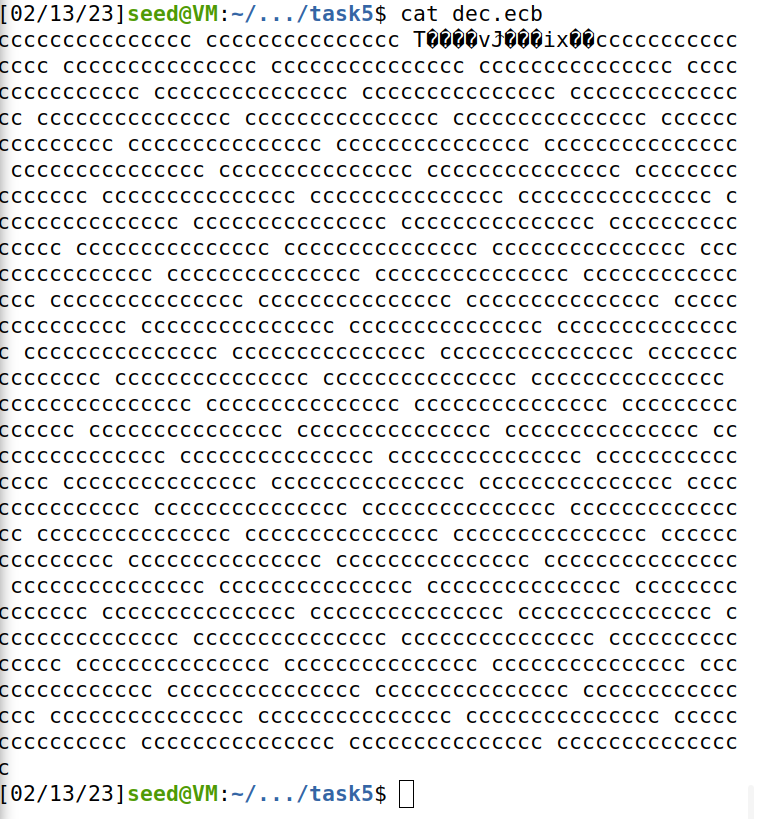
\includegraphics[height=\textheight,width=\textwidth,keepaspectratio]
    {figures/dec_ecb_task5.png}
    \caption{Decrypted text with corrupted bits using ECB mode.}\label{fig:corrupted_ecb}
\end{figure}

\begin{figure}
    \centering
    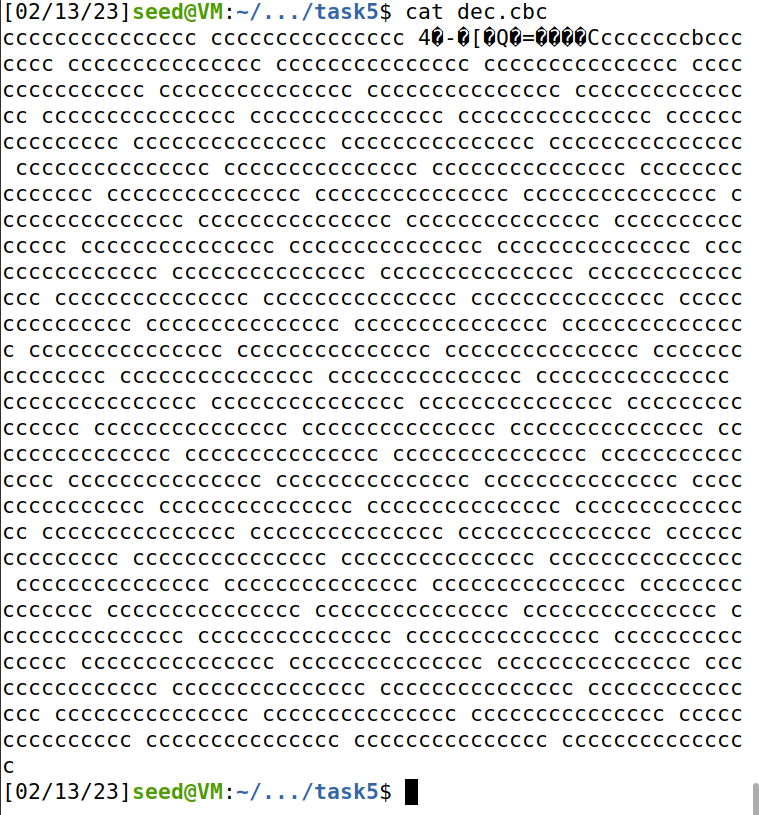
\includegraphics[height=\textheight,width=\textwidth,keepaspectratio]
    {figures/dec_cbc_task5.png}
    \caption{Decrypted text with corrupted bits using CBC mode.}\label{fig:corrupted_cbc}
\end{figure}

\begin{figure}
    \centering
    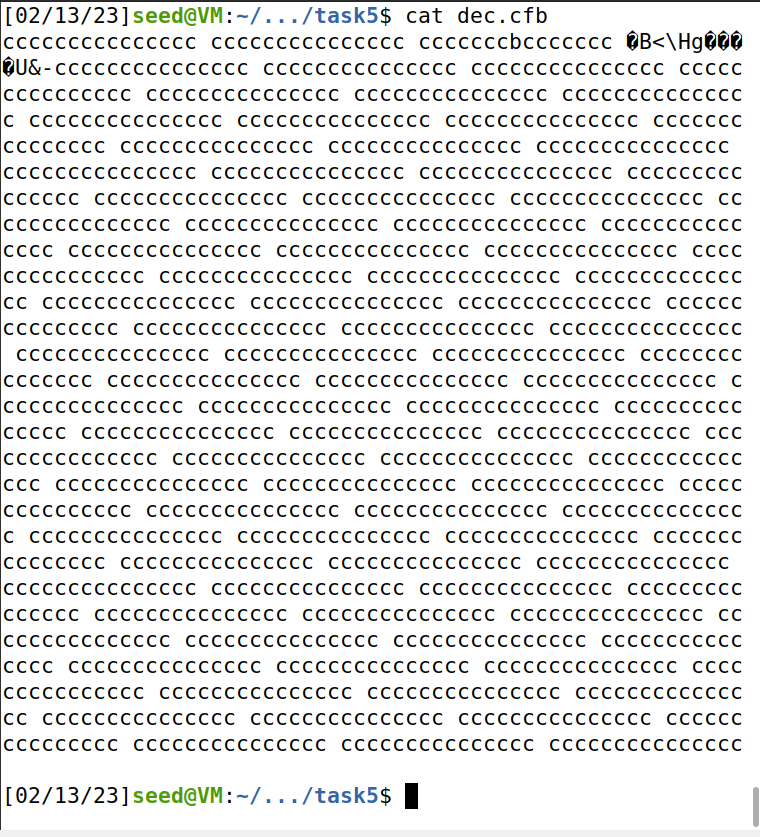
\includegraphics[height=\textheight,width=\textwidth,keepaspectratio]
    {figures/dec_cfb_task5.png}
    \caption{Decrypted text with corrupted bits using CFB mode.}\label{fig:corrupted_cfb}
\end{figure}

\begin{figure}
    \centering
    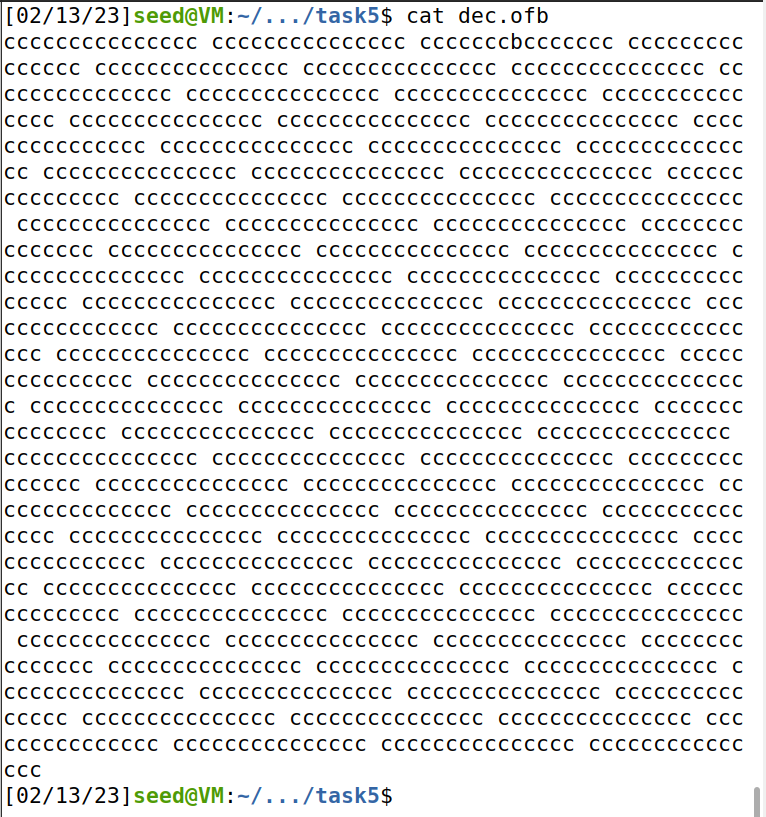
\includegraphics[height=\textheight,width=\textwidth,keepaspectratio]
    {figures/dec_ofb_task5.png}
    \caption{Decrypted text with corrupted bits using OFB mode}\label{fig:corrupted_ofb}
\end{figure}

\begin{figure}
    \centering
    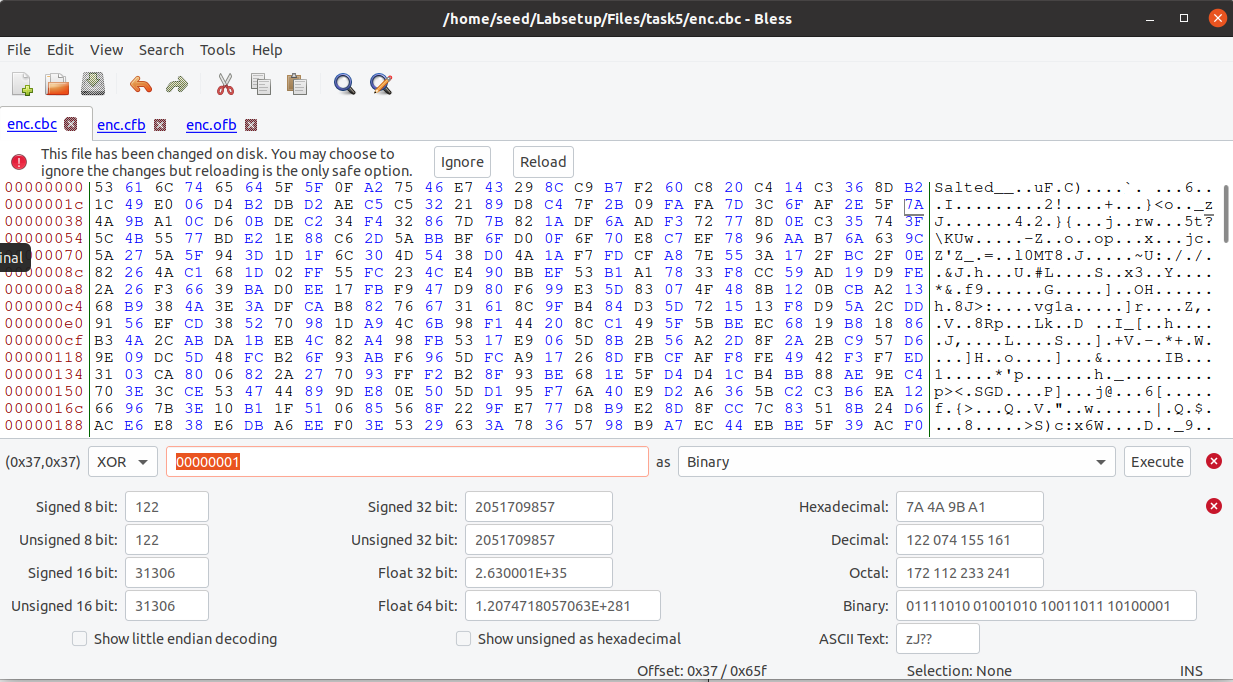
\includegraphics[height=\textheight,width=\textwidth,keepaspectratio]
    {figures/bless_editor.png}
    \caption{Modify the \(55^{th}\) bit using Bless hex editor.}
    \label{fig:bless_editor}
\end{figure}

\begin{figure}
    \centering
    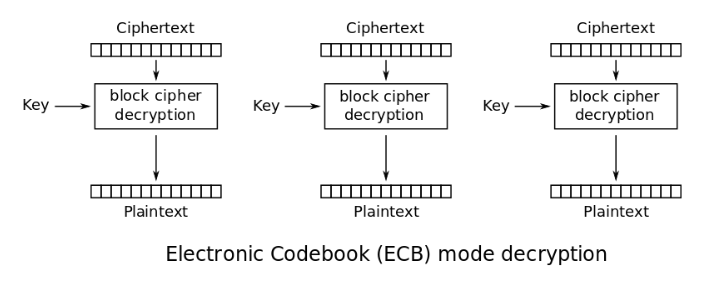
\includegraphics[height=\textheight,width=\textwidth,keepaspectratio]
    {figures/ecb_decryption.png}
    \caption{ECB mode decryption}\label{fig:ecb_dec}
\end{figure}

\begin{figure}
    \centering
    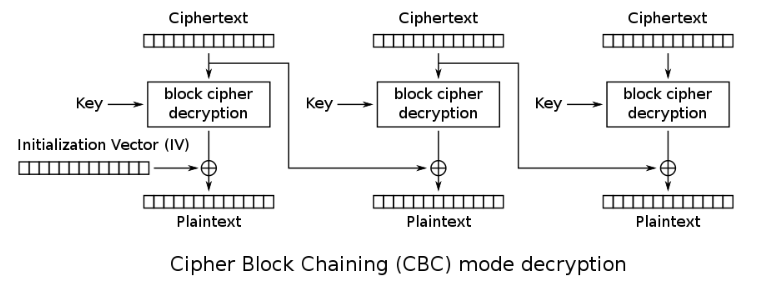
\includegraphics[height=\textheight,width=\textwidth,keepaspectratio]
    {figures/cbc_decryption.png}
    \caption{CBC mode decryption}\label{fig:cbc_dec}
\end{figure}

\begin{figure}
    \centering
    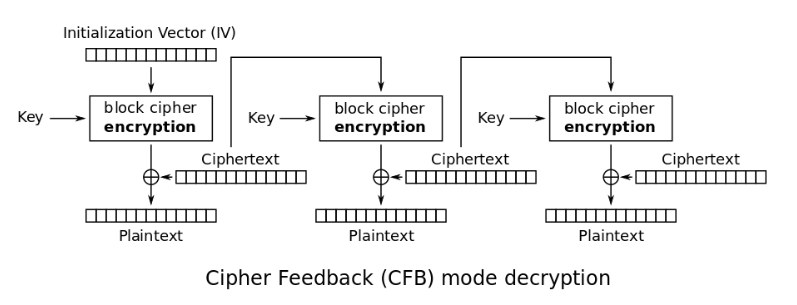
\includegraphics[height=\textheight,width=\textwidth,keepaspectratio]
    {figures/cfb_decryption.png}
    \caption{CFB mode decryption}\label{fig:cfb_dec}
\end{figure}

\begin{figure}
    \centering
    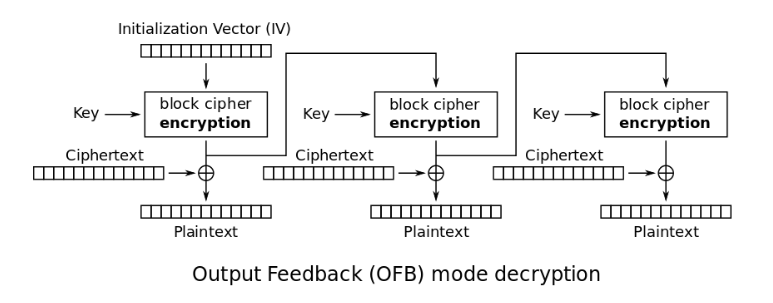
\includegraphics[height=\textheight,width=\textwidth,keepaspectratio]
    {figures/ofb_decryption.png}
    \caption{OFB mode decryption}\label{fig:ofb_dec}
\end{figure}

At first, we created a {\fontfamily{qcr}\selectfont plaintext.txt} that is 1600 bytes long
(see \autoref{lst:plaintext_generation}). The plaintext should be like a chain of strings
``ccccccccccccccc '' (15 `c' characters with a space at the end).
After encrypting it with AES-128 cipher, we used
{\fontfamily{qcr}\selectfont bless} hex editor to modify the \(55^{th}\) byte of the
encrypted file. We did XOR the \(55^{th}\) byte with {\fontfamily{qcr}\selectfont 00000001}
to flip the least significant bit (see \autoref{fig:bless_editor}). Next, we decrypted
files to observe how bit errors behave.

In ECB mode (see \autoref{fig:corrupted_ecb}, \autoref{fig:ecb_dec}), a whole block (16 bytes)
is changed (different
from the original plaintext). Each blocks are decrypted separately as shown in
\autoref{fig:ecb_dec}. Thus, only the block containing the corrupted bit is affected. And
the ciphertext block is fed into the decryptor, so with many substitution, extension, and
permutation steps are performed within the decryptor, the corrupted bits are spread to the
whole block.

In CBC mode (see \autoref{fig:corrupted_cbc}, \autoref{fig:cbc_dec}), the block which holds
the corrupted bit
is changed totally as ciphertext block is fed into the decryptor. However, the next block
is changed at the specific bit according to the position we modified since the current ciphertext
block is only XORed with the output of decryptor of the next block (not being fed into
a decryptor of the next block). In this case, the original character `c' is changed to
`b' as a result of flipping the least significant bit.

In constrast to CBC mode, in CFB mode, the block which holds the corrupted bit changed at a specific
bit according to the position we modified as the corrupted ciphertext block is only XORed
with the output of the decryptor (see \autoref{fig:corrupted_cfb}, \autoref{fig:cfb_dec}).
However, the next block is changed totally as the corrupted ciphertext block is fed into
the decryptor of the next block.

In OFB mode (see \autoref{fig:corrupted_ofb}, \autoref{fig:ofb_dec}), only the current block
is changed at the specific bit according to the position we modified as the corrupted ciphertext
block is only XORed with the output of the decryptor, not being sent to the next block.

After collecting the observations from above tasks and referencing some sources, we created
\autoref{tab:error_effect} to illustrate exactly the effect of bit errors. In that table,
\(C_i\) is the \(i^{th}\) ciphertext block, and \(P_i\) is the \(i^{th}\) plaintext block.
We can conclude that our prediction before experiments and the observation matches each
other.

\begin{table}
    \centering
    \begin{tabular}{|l|l|}
        \hline
        Mode & Effect of Bit Errors in \(C_i\)\\
        \hline
        ECB & Random bit errors in \(P_i\)\\
        \hline
        CBC & Random bit errors in \(P_i\)\\
         & Specific bit errors in \(P_{i+1}\)\\
        \hline
        CFB & Specific bit erros in \(P_i\)\\
         & Random bit errors in \(P_{i+1},P_{i+2},\cdot,\) until synchronization is restored.\\
        \hline
        OFB & Specific bit errors in \(P_i\)\\
        \hline
    \end{tabular}
    \caption{The effect of bit errors for block cipher modes~\cite{cipher_mode_wiki,error_prop}.}
    \label{tab:error_effect}
\end{table}
